% Generated by scripts/supp_tex.py from scripts/supp/c_derivations.py.
% Do not edit: edit the module, which also builds the PDF version.

\section{Derivations}
\label{supp:c_derivations}

This section states the allocation problem from its objects upward and proves what the paper asserts about it. Nothing here needs a result from elsewhere in the supplement. Each statement carries the assumptions it uses, a proof, and a remark on what it leaves open.

\begin{table}[t]
\centering
\resizebox{\columnwidth}{!}{%
\begin{tabular}{lrrrr}
\toprule
no. & claim & in & checked in & ckpt \\
\midrule
P1 & separates over tiles & A.2 & verify\_theory & eval \\
P2 & monotone in $\lambda$ & A.2 & verify\_theory & eval \\
P3 & blind sets are a hull & A.3 & static\_RECIPE512\_b01 & PAPER \\
T4 & a Minkowski average & A.3 & not measured & - \\
P5 & reaches only the hull & A.3 & hull\_gap & eval \\
P6 & savings on a 1/N lattice & A.3 & theory\_checks & eval \\
P7 & the floor & A.4 & saturation\_RECIPE512 & PAPER \\
P8 & the saturation price & A.4 & verify\_theory & eval \\
P9 & the ceiling & A.4 & per\_class\_RECIPE512 & PAPER \\
T10 & adaptivity gain & A.5 & theory\_check & BEST \\
P11 & plotted log-convexity & A.6 & logconvexity & none \\
P12 & Lorenz bound & A.7 & hybrid\_RECIPE512\_b01 & PAPER \\
P13 & rank-1 threshold rule & A.8 & raterank\_RECIPE512\_b01 & PAPER \\
P14 & rank-1 uses hull exits & A.8 & raterank\_RECIPE512\_b01 & PAPER \\
\bottomrule
\end{tabular}}
\caption{\textbf{The numbered results of this section, and the evidence for each.} P is a proposition and T a theorem; the numbering is stable and is what the main paper cites. PAPER is runs/RECIPE512/ckpt\_PAPER.pth.tar, eval is runs/RECIPE512/ckpt\_eval.pth.tar and BEST is runs/BEST/ckpt\_eval.pth.tar. verify\_theory is scripts/verify\_theory.py, which reports seven of seven propositions passing on one sequence at one rate.}
\end{table}

{\small Files named without a directory are under results/ with a .json extension; the saturation and Lorenz rows are the \_ctc53 and \_b01\_fixed variants of the names given. T4 is proved and not measured: it describes a set of 120 vertices that no experiment enumerates.}

\subsection{The setting, and four assumptions}

\textbf{Tiles.} The decoder is cut at a fixed depth: everything above the cut runs once over the whole frame, everything below on square patches of the trunk's feature grid. Replicate padding makes the grid divide exactly, so the tiling is a partition. Tiles are indexed by t and N is their number in a frame, 40 at 1080p and 2 at 416$\times$240; section A gives their geometry.

\textbf{Exits.} An exit is a point at which a tile may stop and be handed to the reconstruction head. There are K = 6 over 12 residual blocks, evenly spaced, so exit k runs (k+1)b blocks with b = 2. At a split depth of j = 2 the first jb blocks run full-frame whatever exit a tile takes, so the usable ladder has K - j = 4 members and k ranges over j, ..., K-1 throughout.

\textbf{Distortion.} D$_{t,k}$ is the mean squared error tile t incurs when it leaves at exit k, measured on the deployed tiled path so that what tiling costs sits inside it, and measured against the released decoder's decode of the same latent so that synthesis is the only difference between the two sides. Nothing forces D$_{t,K-1}$ to zero, and A.4 returns to that.

\textbf{Decibels.} Distortion is reported as 10 log$_{10}$ of the ratio to the reference, and the ratio can be formed at two levels. Pooling every tile of every frame into one mean squared error is the form the Lagrangian below is exact for; averaging a per-frame decibel is the codec convention, and it is what the budget is bisected against throughout. Section E measures how far apart the two read on one allocation, which is a substantial fraction of the working budget.

\textbf{Compute.} Compute is counted in multiply-accumulate operations and divided by those of one released full-frame decode, \IntraGmac\,GMAC at 1080p, so c = 1 is one released decode and a saving of S\% means the frame was decoded for (1 - S/100) of one. Every operator runs at a fixed multiple of the latent grid, which makes the cost of an exit resolution-independent. One tile at exit k costs

\begin{equation}
c_k \;=\; s_{\mathrm{up}} \;+\; s_{\mathrm{trunk}}\,\frac{(k+1)\,b}{N_{\mathrm{blk}}} \;+\; s_{\mathrm{head}} \;+\; a_k \;+\; r,
\end{equation}

with s$_{up}$ the opening upsample, s$_{trunk}$ the trunk spread over N$_{blk}$ = 12 blocks of which exit k runs (k+1)b, s$_{head}$ the head, a$_{k}$ the adapter exit k wears and r the full-frame deblocking filter; section B measures all five. Only the trunk term depends on k, which is why a ceiling exists: however shallow the ladder gets, the stem, the head and the filter are still paid.

\begin{table}[t]
\centering
\resizebox{\columnwidth}{!}{%
\begin{tabular}{lrrrrrr}
\toprule
exit k & blocks & adapter & share & c\_k & 100(1-c\_k) & c\_k, stored \\
\midrule
2 & 6 & ffn & 0.712 & 0.6088 & 39.12 & 0.5809 \\
3 & 8 & ffn & 0.712 & 0.7578 & 24.22 & 0.7300 \\
4 & 10 & 1$\times$1 & 0.142 & 0.8697 & 13.03 & 0.8697 \\
5 & 12 & none & 0.000 & 1.0095 & -0.95 & 1.0095 \\
\bottomrule
\end{tabular}}
\caption{\textbf{What each exit costs}, in units of one released full-frame decode, with the adapter share in units of one residual block. The deepest exit costs more than 1 because a tiled decode still pays the deblocking filter. The last column is the cost vector stored in results/tile\_table.json, which is the one the checks of Propositions 5, 6, 8 and 10 are computed on; each says so where it appears.}
\end{table}

{\small c\_k from the uniform-depth rows of results/static\_RECIPE512\_b01.json and adapter shares from results/adapter\_cost.json, both on runs/RECIPE512/ckpt\_PAPER.pth.tar. Section B audits the block count itself and prices the gap between the model the argmin runs on and the hook count every saving is quoted from.}

The gaps between those costs are what the allocation trades in, and they are unequal: 0.1491, 0.1119 and 0.1398. The first is largest because exit 3 gives up the FFN adapter's saving as well as two blocks.

\textbf{Assignments.} An assignment is a map a from tiles to exits. There are (K-j)$^{N}$ of them, 4$^{40}$ at 1080p, so they will not be enumerated. The frame's compute and distortion are

\begin{equation}
C(a) \;=\; \frac{1}{N}\sum_{t=1}^{N} c_{a(t)}, \qquad D(a) \;=\; \frac{1}{N}\sum_{t=1}^{N} D_{t,a(t)}.
\end{equation}

Everything after this rests on four assumptions, none of them a mathematical necessity. Each result names the ones it uses.

\begin{itemize}\itemsep1pt
\item \textbf{(A1) Compute is additive over tiles.} Exact when tiles decode independently, which is what a tiled decoder does.
\item \textbf{(A2) Distortion is a tile mean}, and a tile's error does not depend on which exits its neighbours took. The first half is exact for any per-pixel loss averaged over a frame; the second is not free, the deblocking filter running on the stitched canvas and seeing the whole exit map at once.
\item \textbf{(A3) The reference is fixed.} D$_{t,k}$ is measured on the deployed tiled path against the released decoder's own decode of the same latent, so rate is identical on both sides and cancels.
\item \textbf{(A4) The cost vector is strictly increasing} in k over k $\geq$ j, which Table 2 shows it is.
\end{itemize}

The second half of (A2) is checked rather than asserted, over 60 allocations of one frame spanning savings of 1.2\% to 41.9\%: the largest disagreement between the per-tile prediction and a decode of the mixed map is 5.5$\times$10$^{-5}$ dB, four orders of magnitude below the budget. Nothing in (A1) to (A4) constrains D$_{t,k}$ itself, and nothing requires it to fall as k grows.

{\small Additivity check computed from results/tile\_table.json (Bosphorus, q32, 40 tiles), checkpoint runs/RECIPE512/ckpt\_eval.pth.tar. What it checks is a property of the decode path rather than of the weights.}

\subsection{A price on compute}

The encoder's problem is to spend as little compute as possible while staying inside a distortion budget:

\begin{equation}
\min_{a}\; C(a) \quad \mathrm{subject\ to} \quad D(a) \;\leq\; D_{\mathrm{budget}}.
\end{equation}

Constraint (0) couples the tiles: whether a tile can afford to leave early depends on how much of the budget the other 39 have used. The standard way out is to buy the constraint off with a price \lambda $\geq$ 0 charged per unit of compute:

\begin{equation}
L(a,\lambda) \;=\; D(a) + \lambda\,C(a) \;=\; \frac{1}{N}\sum_{t=1}^{N}\left[\,D_{t,a(t)} + \lambda\,c_{a(t)}\,\right].
\end{equation}

\lambda is an exchange rate, in squared error per unit of relative compute, so \lambda c$_{k}$ converts the compute an exit uses into the squared error that compute is deemed to be worth. Below it runs from about 2$\times$10$^{-7}$ to about 1$\times$10$^{-4}$, against squared errors of order 1$\times$10$^{-4}$ on a 0 to 1 scale, and what matters is where it sits relative to the differences between exits: at zero every tile takes its own lowest-error exit, and past a large enough price every tile has dropped as far as the ladder allows.

\paragraph{Proposition 1 (separation)}

For every \lambda $\geq$ 0, an assignment minimises L(a,\lambda) over all assignments if and only if it minimises the bracket tile by tile:

\begin{equation}
k^{\star}_t(\lambda) \;\in\; \mathrm{arg\,min}_{k \geq j}\;\left[\,D_{t,k} + \lambda\,c_k\,\right].
\end{equation}

\emph{Assumes} (A1) and (A2).

\emph{Proof.} Write f$_{t}$(k) = D$_{t,k}$ + \lambda c$_{k}$. Then N L(a,\lambda) = ∑$_{t}$ f$_{t}$(a(t)), a sum in which the t-th term depends on a only through a(t). For any assignment a, term by term f$_{t}$(a(t)) $\geq$ min$_{k}$ f$_{t}$(k), so N L(a,\lambda) $\geq$ ∑$_{t}$ min$_{k}$ f$_{t}$(k), and the right-hand side is attained by any a that picks a minimiser in every tile. Conversely if a is optimal and some tile had f$_{t}$(a(t)) > min$_{k}$ f$_{t}$(k), replacing a(t) by that minimiser and leaving every other tile alone would strictly lower L.

\emph{Remark.} The result is about the frame mean and bounds no single tile. At the deployed 0.1 dB operating point the worst tile in the test set gives up 1.97 dB, so a frame inside its budget can hold a tile an order of magnitude outside it; section D tabulates that tail. No result in this section repairs it.

{\small Per-tile tail from results/supp\_opquality\_PAPER.json, checkpoint runs/RECIPE512/ckpt\_PAPER.pth.tar, at the operating point read from results/signalled\_RECIPE512\_ctc53.json.}

The N-dimensional search has become N independent searches over 4 numbers each, with ties broken toward the shallower exit so that k$^{*}$ is a function. We call k$^{*}$$_{t}$(\lambda) the oracle's choice, because it uses the true D$_{t,k}$, which only the encoder has. The construction is Shoham and Gersho's [26] with compute in place of rate, made standard in coding by [27].

\paragraph{Proposition 2 (monotonicity)}

Let \lambda$_{1}$ < \lambda$_{2}$ and let a$_{1}$, a$_{2}$ be the corresponding oracle assignments. Then C(a$_{2}$) $\leq$ C(a$_{1}$) and D(a$_{2}$) $\geq$ D(a$_{1}$). \emph{Assumes} (A1), (A2) and Proposition 1.

\emph{Proof.} Fix a tile and drop the index. Optimality at each price gives D$_{1}$ + \lambda$_{1}$c$_{1}$ $\leq$ D$_{2}$ + \lambda$_{1}$c$_{2}$ and D$_{2}$ + \lambda$_{2}$c$_{2}$ $\leq$ D$_{1}$ + \lambda$_{2}$c$_{1}$, where (D$_{i}$, c$_{i}$) is the pair chosen at \lambda$_{i}$. Adding the two and cancelling D$_{1}$ + D$_{2}$ leaves (\lambda$_{2}$ - \lambda$_{1}$)(c$_{2}$ - c$_{1}$) $\leq$ 0, hence c$_{2}$ $\leq$ c$_{1}$. Substituting that back into the first inequality gives D$_{2}$ $\geq$ D$_{1}$ + \lambda$_{1}$(c$_{1}$ - c$_{2}$) $\geq$ D$_{1}$. Averaging over tiles preserves both.

\emph{Remark.} Monotone is not continuous. Cost moves in the jumps Proposition 6 measures, so bisecting \lambda converges on a reachable level rather than on the budget. The result also assumes exact minimisation of the true table, whereas the deployed search bisects a predicted table and corrects with a real decode, at most six passes to 5$\times$10$^{-4}$ dB.

\begin{table}[t]
\centering
\resizebox{\columnwidth}{!}{%
\begin{tabular}{lrrrrrr}
\toprule
tile & bits & D(2) & D(3) & D(4) & D(5) & exits as $\lambda$ rises \\
\midrule
34 & 10,446 & 1.608 & 1.638 & 1.679 & 1.655 & 2 throughout \\
0 & 12,996 & 9.346 & 9.249 & 9.207 & 9.180 & 5, 4 at 1.9, 3 at 3.0, 2 at 6.5 \\
18 & 16,989 & 16.249 & 15.795 & 15.638 & 15.606 & 5, 4 at 2.3, 3 at 11.2, 2 at 30.6 \\
\bottomrule
\end{tabular}}
\caption{\textbf{Three tiles of one frame, and what the price does to them.} D is in units of 10$^{-5}$ squared error and switch points in units of 10$^{-6}$ of $\lambda$. The cheapest tile prefers the shallowest exit at every price including $\lambda$ = 0, its error not falling with depth at all, so depth is not always worth buying. The most expensive tile holds out against the shallowest exit 4.7 times longer than the middle one, which is why one uniform depth cannot suit both.}
\end{table}

{\small results/tile\_table.json (Bosphorus, q32, 40 tiles), checkpoint runs/RECIPE512/ckpt\_eval.pth.tar. The 60 prices stored in that file produce 33 distinct savings, the granularity A.3 quantifies.}

\subsection{The achievable set, and what one price reaches}

The pairs (C(a), D(a)) an allocation can produce form a set whose shape decides both what a sweep can reach and what adaptivity is worth. There are two versions of it. Write

\begin{equation}
\bar D_k \;=\; \frac{1}{N}\sum_{t=1}^{N} D_{t,k},
\end{equation}

for the exit mean at k, the one place tiles are averaged before anything is chosen.

\paragraph{Proposition 3 (fixed proportions)}

Suppose tiles are assigned to exits in proportions p, one probability per exit, independently of their content. Then the achievable set of expected pairs is exactly the convex hull of the K-j points whose coordinates are the cost c$_{k}$ and the exit mean at k. \emph{Assumes} (A1) and (A2).

\emph{Proof.} Under content-independent proportions the expected cost is ∑$_{k}$ p$_{k}$ c$_{k}$ and, by the tile mean, the expected distortion is ∑$_{k}$ p$_{k}$ times the exit mean at k. The map from p to that pair is affine and its domain is the probability simplex, whose extreme points are the unit vectors. An affine image of a simplex is the convex hull of the images of its vertices, and those images are the cost and exit mean of each exit.

\emph{Remark.} The hull is a hull of expectations. One frame with N tiles realises proportions in multiples of 1/N, so interior points are attained only to that granularity, and at N = 2 the smallest test class reaches three mixtures per pair of exits.

The four uniform-depth decodes are the vertices of that hull, and they are everything a content-blind allocation can reach; section D tabulates them in dB at every rate beside the two shuffled controls. The mean over rates of the best single depth is \BestStaticMean\%, against \MainMean\% for the per-tile allocation at the same budget.

{\small results/static\_RECIPE512\_b01.json, checkpoint runs/RECIPE512/ckpt\_PAPER.pth.tar, \NumSeq frames.}

\paragraph{Theorem 4 (per-tile assignment)}

The convex hull of the pairs achievable by per-tile assignment is the Minkowski average of the N per-tile hulls,

\begin{equation}
\mathcal{A}_{\mathrm{tile}} \;=\; \frac{1}{N}\bigoplus_{t=1}^{N}\mathrm{conv}\{(c_k, D_{t,k}) : k \geq j\}.
\end{equation}

\emph{Assumes} (A1) and (A2).

\emph{Proof.} By (A1) and (A2) an achievable pair is the average of one point drawn from each per-tile set S$_{t}$, the set of pairs cost c$_{k}$ against error D$_{t,k}$, so the achievable set is the Minkowski average of the S$_{t}$. Taking convex hulls commutes with Minkowski addition, the hull of a sum being the sum of the hulls, and with positive scaling; applying that N-1 times moves the hull inside the sum.

\emph{Remark.} The theorem bounds what any allocation reaches, a perfect router included, and says nothing about which of those points a price reaches, which is Proposition 5. It is the one result here with no measurement behind it, the set having up to N(K-j-1) = 120 vertices at 1080p.

Proposition 3 is the special case in which every tile has the same row, and otherwise the per-tile set is strictly larger: the fixed-proportion hull has at most K-j = 4 vertices and so 3 straight segments, while the Minkowski average is smooth at any plotted scale. Figure 1 draws both on one frame.

\begin{figure}[t]
\centering
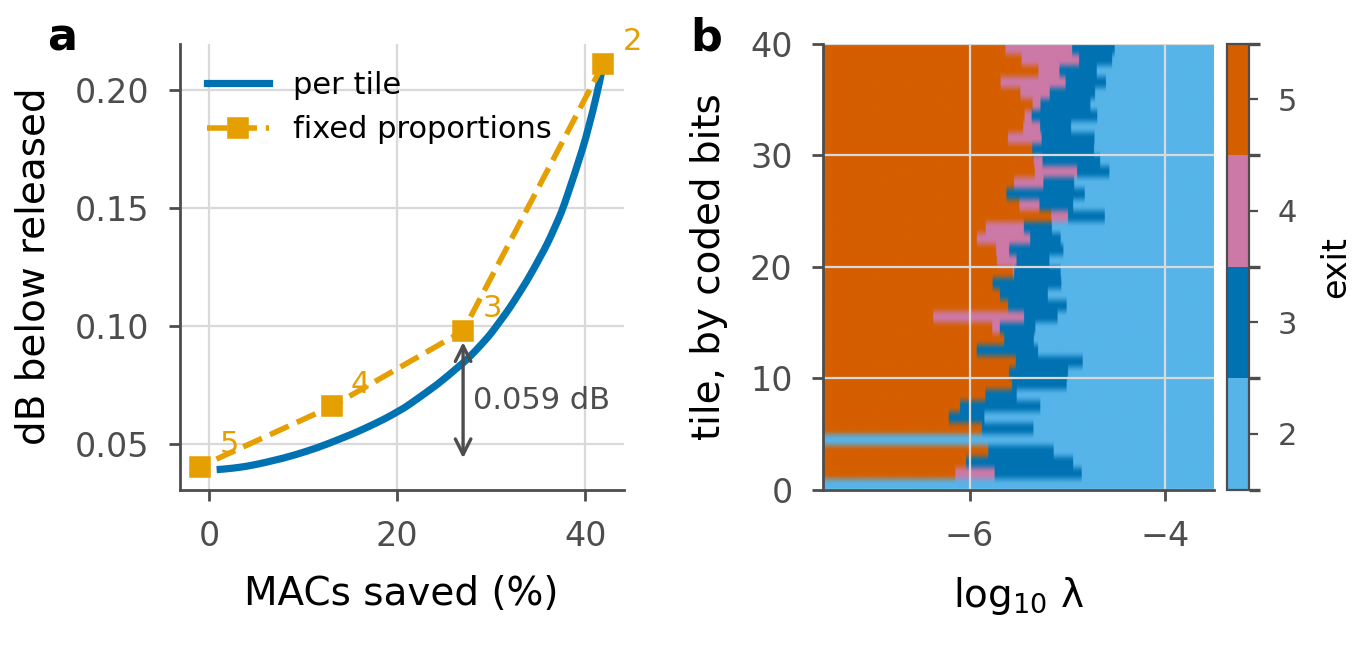
\includegraphics[width=\columnwidth]{figures/supp_achievable.png}
\caption{\textbf{The two achievable sets, on one frame.} \textbf{a}, the per-tile frontier of Theorem 4 traced by sweeping $\lambda$, against the fixed-proportion chain of Proposition 3 through the four uniform-depth points, labelled by exit. The per-tile curve lies below the chain everywhere between the vertices, by 0.059 dB at the exit-3 vertex. \textbf{b}, the exit each of the 40 tiles takes as $\lambda$ rises, tiles ordered by the bits the entropy coder spent on them. Every row is non-increasing, which is Proposition 2 per tile, and the rows differ, which is what Theorem 4 buys over Proposition 3. The bottom row is a tile that never leaves the shallowest exit.}
\end{figure}

{\small Both panels from results/tile\_table.json (Bosphorus, q32, 40 tiles), checkpoint runs/RECIPE512/ckpt\_eval.pth.tar, drawn by scripts/supp\_derivations\_figure.py on that file's own cost vector, the last column of Table 2. A grid of 4001 prices finds 93 distinct reachable savings on this frame, against the 95 the dynamic programme of Table 4 enumerates.}

\paragraph{Proposition 5 (a price reaches only the lower hull)}

For every \lambda $\geq$ 0 the point (C, D) produced by the oracle assignment lies on the lower convex hull of the achievable set, and no \lambda produces a point strictly inside it. \emph{Assumes} (A1), (A2) and Proposition 1.

\emph{Proof.} By Proposition 1 the oracle assignment minimises D(a) + \lambda C(a) over all assignments, so its pair minimises the linear functional (C, D) $\rightarrow$ D + \lambda C over the achievable set and hence over that set's convex hull. A minimiser of a linear functional over a compact convex set lies on its boundary, and because \lambda $\geq$ 0 the supporting line has slope -\lambda $\leq$ 0, which places the point on the lower boundary. Conversely a point strictly inside the hull is a strict convex combination of achievable points and is therefore strictly beaten, at that same C, by some point of the hull, so it cannot minimise any such functional.

\emph{Remark.} A budget between two hull vertices is unreachable by any price, and the proposition does not say what that costs, which is Proposition 6. The measurement below enumerates the exact Pareto set on one frame at one rate, on that file's own cost vector.

Everett's generalised multiplier method (1963) supplies the reassuring half of the converse: whatever compute the returned allocation consumes, it is optimal for that level. With four distinct exit costs the whole Pareto set can be enumerated by dynamic programming over tiles, so the other half can be priced exactly.

\begin{table}[t]
\centering
\resizebox{\columnwidth}{!}{%
\begin{tabular}{lrrr}
\toprule
budget dB & by sweep & exact Pareto & gap \\
\midrule
0.05 & 12.398 & 12.421 & 0.0230 \\
0.08 & 25.443 & 25.489 & 0.0452 \\
0.10 & 30.475 & 30.496 & 0.0209 \\
0.12 & 33.782 & 33.803 & 0.0211 \\
0.15 & 37.439 & 37.461 & 0.0211 \\
0.18 & 40.048 & 40.046 & -0.0018 \\
0.20 & 41.166 & 41.165 & -0.0016 \\
\bottomrule
\end{tabular}}
\caption{\textbf{What convexity costs.} Savings in per cent at seven budgets on one frame. The sweep reaches 95 allocations against the 635 on the exact Pareto set, and the largest loss over these budgets is 0.045 saving points. The two negative entries are the sweep landing on a budget the enumeration's grid straddles rather than the sweep beating the Pareto set, which Proposition 5 forbids.}
\end{table}

{\small results/hull\_gap.json, Bosphorus q32, 40 tiles. The enumeration and the sweep read one cost vector, so the gap does not depend on which one.}

\paragraph{Proposition 6 (granularity)}

If at most m tiles switch exit at any single breakpoint of the sweep, and each switch moves a tile by one rung, then consecutive reachable savings differ by at most

\begin{equation}
\mathrm{spacing} \;\leq\; \frac{100\;m\,\max_k (c_{k+1}-c_k)}{N}\;\%,
\end{equation}

and the loss from convexity cannot exceed the largest spacing. \emph{Assumes} (A1), (A4) and Proposition 2.

\emph{Proof.} Between breakpoints the assignment is constant, so the reachable costs are exactly the costs at the breakpoints. At one breakpoint the mean cost changes by 1/N times the sum of the individual changes, each at most max$_{k}$(c$_{k+1}$ - c$_{k}$) in magnitude, and there are at most m of them; multiplying by 100 puts it in saving points. For the second part, let a budget fall strictly between two reachable levels. By Proposition 2 the bisection returns the lower level, so the loss is at most the distance between them.

\emph{Remark.} Both hypotheses are read off a measured table rather than guaranteed, and the bound is vacuous if either fails on another frame. It falls as 1/N, so it says nothing useful at the smallest test class, where N = 2 and one switch moves the frame by half the largest rung.

On the measured table m = 2, tiles with identical rows switching together, the largest rung is 0.1491 and N = 40, so the bound is 0.7453 saving points. The measured spacing is 0.7453, sitting on the bound, and the convexity loss of Table 4 is 0.0452. Nothing in the expression depends on content or on rate, and halving the tile side would put four times as many tiles on the lattice, each carrying a quarter of the step.

{\small m, the largest rung, the bound and the measured spacing from results/theory\_checks.json (Bosphorus q32, 40 tiles, runs/RECIPE512/ckpt\_eval.pth.tar), written by scripts/verify\_theory.py.}

\subsection{Floor, saturation and ceiling}

The sweep has two ends, and a budget outside them buys nothing. The budget section measures where they sit at each rate; this one derives them.

\paragraph{Proposition 7 (the floor)}

At \lambda = 0 the allocation attains D$_{min}$ = (1/N) ∑$_{t}$ min$_{k}$ D$_{t,k}$, and no allocation attains less. \emph{Assumes} (A2) and Proposition 1. \emph{Proof.} Immediate from Proposition 1 at \lambda = 0, and from D(a) being a mean of terms each bounded below by its own tile minimum.

\emph{Remark.} The floor is a statement about the table, and the table is a product of training, which (A3) does not constrain. If the deepest exit drifts from the reference by δ then the achievable set shifts up by δ before any compute is saved, and a budget below δ is unreachable at every allocation. Section H measures that drift, with and without the training objective's anchor term.

Because D$_{t,k}$ is measured on the deployed tiled path, D$_{min}$ is not zero: it is what tiling costs before any tile exits early, and section E measures where it sits at each rate and which budgets fall below it.

\paragraph{Proposition 8 (saturation)}

Define

\begin{equation}
\lambda_{\mathrm{sat}} \;=\; \max_{t}\;\max_{k>j}\;\frac{D_{t,j}-D_{t,k}}{c_k-c_j},
\end{equation}

Then for every \lambda > \lambda$_{sat}$ the oracle assigns exit j to every tile, the frame's cost is exactly c$_{j}$, and no larger price changes anything. \emph{Assumes} (A1), (A4) and Proposition 1.

\emph{Proof.} Exit j beats exit k on tile t precisely when D$_{t,j}$ + \lambda c$_{j}$ $\leq$ D$_{t,k}$ + \lambda c$_{k}$, that is when \lambda $\geq$ (D$_{t,j}$ - D$_{t,k}$)/(c$_{k}$ - c$_{j}$), the denominator being positive for k > j by (A4). Taking the maximum over k and then over t gives a single price beyond which exit j wins everywhere. The cost of the constant map is c$_{j}$ by (0).

\emph{Remark.} \lambda$_{sat}$ is a maximum over the tiles of one frame, so a price chosen for a sequence saturates some of its frames and not others, and it constrains the price rather than the budget. On the worked frame the closed form gives 3.045$\times$10$^{-5}$, exactly the last switch of the most expensive tile in Table 3.

\paragraph{Proposition 9 (the ceiling)}

The largest saving any allocation can reach is

\begin{equation}
S_{\max} \;=\; 100\,(1-c_j)\,\%.
\end{equation}

\emph{Assumes} (A1), (A4) and Proposition 8. \emph{Proof.} C(a) is a mean of costs each at least c$_{j}$, j being the shallowest usable exit, so C(a) $\geq$ c$_{j}$ with equality only for the constant map, which Proposition 8 shows is attained.

\emph{Remark.} S$_{max}$ depends on the split depth alone, so no amount of training raises it and the only lever is j. It is a ceiling in multiply-accumulates and not in seconds, and section B reports the wall clock falling short of it. Over the 18 class-and-rate cells measured at a saturating budget it spreads by 6e-06 saving points, which is single-precision noise.

{\small Per-class invariance from results/per\_class\_RECIPE512.json at budgets of 0.5 dB and above, checkpoint runs/RECIPE512/ckpt\_PAPER.pth.tar; the ceiling itself is \CeilingModelled\%, from results/saturation\_RECIPE512\_ctc53.json.}

\subsection{What adaptivity is worth}

What content awareness is worth can be answered without building a predictor. Compare the best per-tile allocation with the best content-blind one at the same price:

\begin{equation}
J_{\mathrm{ad}}(\lambda)=\frac{1}{N}\sum_{t}\min_{k}\left[D_{t,k}+\lambda c_k\right], \quad J_{\mathrm{fix}}(\lambda)=\min_{k}\left[\bar D_k+\lambda c_k\right].
\end{equation}

J$_{ad}$ takes the minimum inside the average and J$_{fix}$ takes it outside. By Propositions 1 and 3 the first is the best the per-tile family attains at price \lambda and the second the best the fixed-proportion family attains.

\paragraph{Theorem 10 (adaptivity gain)}

For every \lambda $\geq$ 0, \Delta(\lambda) = J$_{fix}$(\lambda) - J$_{ad}$(\lambda) $\geq$ 0, with equality if and only if some single exit k$^{*}$ attains the per-tile minimum for every tile. \emph{Assumes} (A1) and (A2).

\emph{Proof.} Fix \lambda and let k be any exit. Then the exit mean at k plus \lambda c$_{k}$ = (1/N) ∑$_{t}$ [D$_{t,k}$ + \lambda c$_{k}$] $\geq$ (1/N) ∑$_{t}$ min$_{k′}$[D$_{t,k′}$ + \lambda c$_{k′}$] = J$_{ad}$(\lambda), because each summand dominates the corresponding minimum. The right-hand side does not depend on k, so taking the minimum over k on the left preserves the inequality and gives J$_{fix}$ $\geq$ J$_{ad}$. For equality, suppose some k$^{*}$ attains the per-tile minimum everywhere; then choosing it makes every summand equal to its minimum and the inequality is tight. Conversely suppose \Delta = 0 and let k$^{*}$ attain J$_{fix}$. Then (1/N) ∑$_{t}$ ([D$_{t,k*}$ + \lambda c$_{k*}$] - min$_{k′}$[D$_{t,k′}$ + \lambda c$_{k′}$]) = 0. Every summand is non-negative, so every summand is zero, which says exactly that k$^{*}$ attains the minimum on every tile.

\emph{Remark.} \Delta upper-bounds what any predictor gains over a content-blind allocation at that price and says nothing about whether one can get any of it, which is what A.7 measures. It is a property of the ladder as much as of the content: improving the shallow exits makes more tiles agree on the argmin, so \Delta falls even as the saving rises and is not a figure of merit.

Read as a ratio $\Delta$/J$_{ad}$ rather than in saving points, the gain rises with rate at a low price and falls to 0.00\% to 0.03\% at the highest price measured, which is Theorem 10's equality condition arriving: the oracle has itself collapsed onto one exit and nothing is left for a router to recover.

{\small Ratios from results/theory\_check.json, checkpoint runs/BEST/ckpt\_eval.pth.tar, 40 sequences (UVG, MCL-JCV and HEVC class E; classes B, C and D not measured), on the last column of Table 2. The table below is the same quantity in saving points on the pinned checkpoint.}

\begin{table}[t]
\centering
\resizebox{\columnwidth}{!}{%
\begin{tabular}{lrrrrr}
\toprule
q & blind \% & oracle \% & gap & blind dB & shuffled dB \\
\midrule
q0 & 25.38 & 29.90 & 4.52 & 0.1262 & 0.1248 \\
q16 & 19.45 & 25.63 & 6.18 & 0.1278 & 0.1335 \\
q32 & 15.02 & 20.93 & 5.91 & 0.1304 & 0.1411 \\
q48 & 12.00 & 18.28 & 6.27 & 0.1373 & 0.1451 \\
q63 & 8.05 & 15.62 & 7.57 & 0.1367 & 0.1413 \\
\bottomrule
\end{tabular}}
\caption{\textbf{The same gap in the units the paper reports.} Columns 2 to 4 are savings at a 0.1 dB budget: the best content-blind mixture of uniform depths, the per-tile oracle, and the difference. Columns 5 and 6 are decibels at the oracle's own compute, what the best blind mixture would read there and what a random shuffle of the oracle's exit map actually reads. Adaptivity is worth 4.5 to 7.6 saving points, rising with rate, against an oracle reading \OracleDb dB and a shuffle reading up to \RandomDb dB.}
\end{table}

{\small Computed from results/static\_RECIPE512\_b01.json, checkpoint runs/RECIPE512/ckpt\_PAPER.pth.tar, \NumSeq frames. The blind columns are the lower hull of the four uniform-depth points under Proposition 3, evaluated at the budget and at the oracle's compute; the shuffle column is a measured decode. At q0 the shuffle reads slightly better than the hull predicts, which bounds the interaction (A2) ignores at under 0.002 dB.}

\subsection{Convexity in the units the frontier is plotted in}

Theorem 4 gives D convex in C. The frontier is almost never plotted in those units: it is plotted as decibels against percentage saving, where convexity is a different statement, the logarithm being concave and increasing and so preserving neither convexity nor concavity. With S = 1 - C/c$_{K-1}$,

\begin{equation}
\mathrm{dB}(S) \;=\; \frac{10}{\ln 10}\,\ln D(C), \qquad C = (1-S)\,c_{K-1}.
\end{equation}

\paragraph{Proposition 11 (plotted convexity is log-convexity)}

Let D be twice differentiable along the frontier. Then dB(S) is convex if and only if D is log-convex in C:

\begin{equation}
D\,D^{\prime\prime} \;\geq\; (D^{\prime})^{2} \qquad\Longleftrightarrow\qquad \frac{d}{dC}\left(\frac{1}{\lambda}\right) \;\geq\; \frac{1}{D}.
\end{equation}

\emph{Assumes} twice differentiability along the frontier, and Proposition 5 for the second form.

\emph{Proof.} C is affine in S and convexity is preserved under affine reparametrisation, so by (0) dB is convex in S if and only if ln D is convex in C. Differentiating twice, (ln D)″ = D″/D - (D′/D)$^2$ = [D D″ - (D′)$^2$]/D$^2$, and D > 0, so (ln D)″ $\geq$ 0 if and only if D D″ $\geq$ (D′)$^2$. For the second form, the slope of the frontier is D′ = -\lambda by the supporting-line argument of Proposition 5, so D″ = -\lambda′; substituting gives -\lambda′ D $\geq$ \lambda$^2$, and dividing by \lambda$^2$ > 0 gives -\lambda′/\lambda$^2$ $\geq$ 1/D, whose left-hand side is d(1/\lambda)/dC. The second form reads as a rate condition: distortion has to fall at least exponentially in compute for the plotted curve to be convex.

\emph{Remark.} This is a property of the decoder rather than a consequence of Theorem 4, and a convex D can fail it. Differentiability fails in one of the two cases: under fixed proportions D is piecewise linear with K-j vertices, so the shape one sees depends on where one samples, whereas the per-tile hull is smooth at any plotted scale.

\begin{table}[t]
\centering
\resizebox{\columnwidth}{!}{%
\begin{tabular}{lrrrr}
\toprule
q & points & condition holds & margin & quartic fit \\
\midrule
q0 & 16 & 100.0\% & 0.0024 & 84.0\% \\
q16 & 14 & 100.0\% & 0.0050 & 76.3\% \\
q32 & 13 & 100.0\% & 0.0088 & 75.3\% \\
q48 & 13 & 100.0\% & 0.0145 & 73.7\% \\
q63 & 13 & 100.0\% & 0.0230 & 74.7\% \\
\bottomrule
\end{tabular}}
\caption{\textbf{Testing log-convexity on the measured frontier.} The direct test asks whether the secant slopes of ln D against S are non-decreasing, and the margin is the smallest increase attained. The condition holds at every point of every frontier and the margin grows tenfold from the lowest rate to the highest. Fitting a quartic and differentiating it twice instead reports 73.7\% to 84.0\%, and the difference is the fit rather than the data: near the ceiling the frontier is close to vertical and a polynomial overshoots, whereas the secant test has no fitted degree to choose.}
\end{table}

{\small results/logconvexity.json. That file records no checkpoint, so it cannot be attributed from disk; its five frontiers have 13 to 16 points each. The quartic column is the file's own quartic\_frac\_ok field.}

\subsection{How much of the oracle a partial signal recovers}

Letting a predictor decide most cases and handing the hardest ones to something exact is the shape of selective prediction [36] and learning to defer [37, 38], and of the budgeted variant of the latter [39]. Two things make the case easier here. The expert is the encoder's own search, exact and free at test time, so what is scarce is the bits needed to say what it decided rather than the expert's time; and the selection rule is not learned, since a separable objective makes the optimal set of size s exactly the s largest regrets. What is left to measure is how concentrated the regret is.

The decoder cannot run the argmin of Proposition 1, D$_{t,k}$ being an error against a source it never receives. A predictor can guess it. Writing p$_{t,k}$ for a head's probability that tile t belongs at exit k, its rule is

\begin{equation}
\hat k_t \;=\; \mathrm{arg\,max}_{k \geq j}\left[\log p_{t,k} - \beta\,c_k\right] \;=\; \mathrm{arg\,min}_{k \geq j}\left[\frac{-\log p_{t,k}}{\kappa} + \lambda\,c_k\right].
\end{equation}

The second form of (0) is the same rule with \beta = \lambda \kappa, \kappa being a fixed calibration turning nats into squared error. Written that way it says that a router is the oracle of (0) with a surrogate in place of D$_{t,k}$, and that one price governs both. Define the per-tile regret at a fixed price:

\begin{equation}
r_t(\lambda) \;=\; \left[D_{t,\hat k_t} + \lambda c_{\hat k_t}\right] - \left[D_{t,k^{\star}_t} + \lambda c_{k^{\star}_t}\right] \;\geq\; 0.
\end{equation}

Non-negativity is immediate from (0). The regret is what the frame's Lagrangian loses on tile t by trusting the prediction, and by Proposition 1 those losses add, so signalling the exits of a subset S removes exactly ∑$_{t∈ S}$ r$_{t}$ from the objective and leaves the rest to the head.

\paragraph{Proposition 12 (Lorenz bound)}

Fix \lambda and let r$_{(1)}$ $\geq$ r$_{(2)}$ $\geq$ ... $\geq$ r$_{(N)}$ be the regrets in decreasing order with total R. For any subset S of size s, the fraction of the total regret that signalling S removes is at most

\begin{equation}
L(\rho) \;=\; \frac{1}{R}\sum_{i=1}^{\lceil \rho N\rceil} r_{(i)}, \qquad \rho = s/N,
\end{equation}

with equality if and only if S is a set of s largest regrets. L is the Lorenz curve of the regret distribution: non-decreasing, concave, running from 0 to 1, and lying above the diagonal by an amount the Gini coefficient summarises. \emph{Assumes} (A1), (A2) and a fixed \lambda.

\emph{Proof.} The sum of any s of the r$_{t}$ is at most the sum of the s largest, since replacing an element of S by a larger one outside S cannot decrease the sum, and repeating that exchange terminates at a set of s largest values. Dividing by R gives the bound. Concavity holds because the increments r$_{(i)}$ are non-increasing by construction.

\emph{Remark.} The bound holds at a fixed price, and the deployed system re-bisects \lambda at every $\rho$ so the frame lands back on its budget. Re-bisecting enlarges the feasible set: the overridden tiles and the predicted ones then carry two multipliers, and pairs of multipliers reach allocations no single one does. The measured recovery is therefore not bounded by L, and Proposition 12 is the wrong thing to call a bound on the deployed system.

\begin{table}[t]
\centering
\resizebox{\columnwidth}{!}{%
\begin{tabular}{lrrrrrrr}
\toprule
q & Gini & L(.1) & rec(.1) & L(.2) & rec(.2) & L(.5) & rec(.5) \\
\midrule
q0 & 0.53 & 35\% & 29\% & 51\% & 53\% & 87\% & 103\% \\
q16 & 0.49 & 27\% & 33\% & 46\% & 59\% & 87\% & 102\% \\
q32 & 0.61 & 37\% & 40\% & 59\% & 68\% & 95\% & 106\% \\
q48 & 0.67 & 45\% & 39\% & 65\% & 63\% & 96\% & 100\% \\
q63 & 0.73 & 53\% & 39\% & 72\% & 62\% & 99\% & 94\% \\
\bottomrule
\end{tabular}}
\caption{\textbf{The Lorenz curve of the regret, and what signalling recovers.} L($\rho$) is the share of the total regret carried by the $\rho$ worst tiles, which Proposition 12 says is the most any signal of that size can remove at a fixed price; rec($\rho$) is the share of the predictor-to-oracle gap the measured sweep recovers. Regret is concentrated at every rate, Gini \GiniMin to \GiniMax: a tenth of the tiles carries 27\% to 53\% of the total regret and recovers 29\% to 40\% of the gap. Over every reachable cell the ratio rec/L runs from \LorenzTightMin\% to \LorenzTightMax\%, for the reason the remark gives.}
\end{table}

{\small results/hybrid\_RECIPE512\_b01\_fixed.json, checkpoint runs/RECIPE512/ckpt\_PAPER.pth.tar, \NumSeq sequences at a 0.1 dB budget; the head it is measured against was trained on runs/RECIPE512/ckpt\_eval.pth.tar. rec($\rho$) is computed here from the same file as the saving at $\rho$, relative to the $\rho$ = 0 and $\rho$ = 1 endpoints. Signalling half the tiles beats signalling all of them at \HybridBeatsAN of \HybridBeatsAOf rates, which is the same re-bisection effect.}

The signal is an entropy-coded mask over tiles plus an index per override, so its bill grows with $\rho$ and is pure overhead at $\rho$ = 1, where the mask names every tile; section G prices both objects. A fifth of the tiles costs \HybridBitsFifth bits per frame and recovers over half the gap.

\subsection{The rate-rank rule, and the model it comes from}

The decoder holds, before the trunk runs, the bits the entropy coder spent on each tile's latents; write b$_{t}$ for that count over the frame's mean. Deriving the rule from a model rather than presenting it as a heuristic says when it must work and how it fails. The model is separability in log space: one scalar difficulty per tile, and one ladder profile applying to every tile in proportion.

\begin{equation}
\log D_{t,k} \;\approx\; u_t + \log\varphi_k, \qquad u_t \;=\; \alpha\log b_t + c.
\end{equation}

Equivalently D$_{t,k}$ = g$_{t}$ $\varphi$$_{k}$ with g$_{t}$ = exp(u$_{t}$) > 0. The profile $\varphi$ is K-j numbers fitted once per rate and \alpha and c are two more, all three fitted leave-one-sequence-out. Nothing is learned per frame and nothing is transmitted, which is why the rule costs the decoder zero.

\paragraph{Proposition 13 (a rank-1 table gives a threshold rule)}

If D$_{t,k}$ = g$_{t}$ $\varphi$$_{k}$ with g$_{t}$ > 0 then

\begin{equation}
\mathrm{arg\,min}_{k \geq j}\left[g_t\varphi_k + \lambda c_k\right] \;=\; \mathrm{arg\,min}_{k \geq j}\left[\varphi_k + \frac{\lambda}{g_t}c_k\right],
\end{equation}

so a tile's exit depends on the tile only through the scalar \lambda/g$_{t}$, and by Proposition 2 the chosen exit is non-increasing in it. Sorting tiles by g$_{t}$ and cutting the sorted list at K-j-1 thresholds therefore reproduces the oracle exactly. \emph{Assumes} exact rank-1 structure, and Proposition 2.

\emph{Proof.} Divide the bracket by g$_{t}$ > 0, which does not move the argmin. The reduced problem is the one-tile problem of (0) with distortion $\varphi$ and price \lambda/g$_{t}$, so Proposition 2 applies and its solution is non-increasing in that price. Since \lambda/g$_{t}$ is decreasing in g$_{t}$, the exit is non-decreasing in g$_{t}$: harder tiles go deeper. The thresholds are the breakpoints of that one common problem and there are at most K-j-1 of them.

\emph{Remark.} Exactness needs an exactly rank-1 table, which no real table is, and the shortfall of the deployed rule measures the departure. The proposition also says the exit is monotone in g$_{t}$ and not that a bit count estimates g$_{t}$, which is a separate and weaker claim.

\paragraph{Proposition 14 (a rank-1 rule uses only the profile's hull)}

Under the same model, an exit k is chosen for some tile at some price only if (c$_{k}$, $\varphi$$_{k}$) lies on the lower convex hull of the profile. \emph{Assumes} exact rank-1 structure, and Propositions 5 and 13. \emph{Proof.} By Proposition 13 the reduced problem is a single Lagrangian sweep over the points (c$_{k}$, $\varphi$$_{k}$), and by Proposition 5 such a sweep reaches only hull points.

\emph{Remark.} The statement is about the fitted profile rather than the true table, so an exit off the hull is dropped by the rule and may still be the oracle's choice. Hull membership is not automatic: on the single-sequence table of results/tile\_table.json the same construction drops exit 4.

Section F prints the fitted $\alpha$ and $\varphi$ at every rate and reports what the rule saves. Two properties of that fit belong here, with the propositions they bear on. $\alpha$ is positive at every rate, so a tile the entropy coder spent bits on is a tile every exit reconstructs worse, and it falls 7-fold from the lowest rate to the highest. And all four exits survive on the lower hull of (c$_{k}$, $\varphi$$_{k}$) at every rate, so Proposition 14 costs nothing here.

{\small Fitted values from results/raterank\_RECIPE512\_b01.json, checkpoint runs/RECIPE512/ckpt\_PAPER.pth.tar, \NumSeq sequences at a 0.1 dB budget; hull membership computed in the build against the shipped cost vector of Table 2.}

The rule gives up \RateRankOracleGap saving points to the Lagrangian oracle at the rate where it does worst, and the loss is not in the separability. On the measured tile table the separable model absorbs 99.96\% of the variance of log D. The quantity it has to resolve is small: the exit profile spans 0.0449 in log units while the non-separable residual has a root mean square of 0.0144, 32\% of it. A model can explain almost all of a table and still be unable to order the differences that decide the argmin, which reads only the differences. Predicting a tile's difficulty from its bit count alone then leaves R$^2$ = 0.84, and by Proposition 13 an error in log g$_{t}$ is a proportional error in the price that tile faces. Coded bits correlate with the mean level of a tile's row at Spearman 0.83 to 0.88 and with the oracle's exit index at 0.39 to 0.54, the ordering the model predicts.

{\small Residual analysis computed from results/tile\_table.json (Bosphorus, q32, 40 tiles), checkpoint runs/RECIPE512/ckpt\_eval.pth.tar; $\alpha$ fitted there is 4.69 against 2.73 for the \NumSeq-sequence fit at the same rate, the difference being one sequence against \NumSeq. Spearman correlations from results/raterank\_RECIPE512\_b01.json, pinned checkpoint; the file stores the last against the negated exit index and it is reported here with the sign flipped, so a positive value means more bits and a deeper exit.}

\subsection{What is proved, what is checked, and what neither covers}

Table 1 lists every result with its evidence. Four gaps in it are worth naming. Theorem 10 is measured as a ratio only on runs/BEST/ckpt\_eval.pth.tar over 40 sequences and on the stored cost vector; the pinned measurement of Table 5 gives it in saving points instead. The convexity check of Table 6 records no checkpoint. The granularity and hull results of A.3 rest on one sequence at one rate, which is enough to check arithmetic and not enough to characterise a codec. And every proposition here concerns a frame mean under (A1) and (A2), so none bounds what a single tile gives up.

